%% Document created 05 March 2021 automatically 
%% from /Users/massimosotgia/Desktop/uni_at_DIFI/Lab_C03/setup.py 

%% Copyright (C) Mattia Sotgia et al. 2021
%% Using class lab_unige.cls
%                                                            
%                                                            
%   **                 **             ******   ****   ****   
%  /**                /**            **////** *///** */// *  
%  /**        ******  /**           **    // /*  */*/    /*  
%  /**       ´´´´´´** /******      /**       /* * /*   ***   
%  /**        ******* /**///**     /**       /**  /*  /// *  
%  /**       **´´´´** /**  /** **  //**    **/*   /* *   /*  
%  /********//********/****** /**   //****** / **** / ****   
%  ////////  //////// /////   //     //////   ////   /´///   
%                                                            
%                                                            
\documentclass[italian, a4paper, 10pt, twocolumn]{../../style/lab_unige}
\usepackage[a4paper, margin=1.25cm, footskip=0.25in]{geometry}

\usepackage[utf8]{inputenc}
\usepackage[T1]{fontenc}

\usepackage[italian]{babel}

% \usepackage{biblatex}

\usepackage[bookmarksopen=true, 
citebordercolor={0 1 0}, 
linkbordercolor={1 0 0}, 
urlbordercolor={0 1 1}]{hyperref}
\usepackage[numbered]{bookmark}

\usepackage{graphicx}
\graphicspath{{../fig/}}
\usepackage{array}
\usepackage{tabulary}
\usepackage{booktabs}

% FOUNDAMENTAL
\usepackage{../../style/custom}

\usepackage{physics}

\usepackage{breqn}
\usepackage{cuted}
\usepackage{txfonts}

\usepackage{lipsum}

%% Define ref types
\newcommand{\reftab}[1]{Tab. {\ref{#1}}}%
\newcommand{\reffig}[1]{Fig. {\ref{#1}}}%
\newcommand{\refeqn}[1]{({\ref{#1}})}%
%% PAPER ONLY custom Macros
\newcommand{\gLab}{$g_t=(9.8056\pm0.0001 \text{ stat}) \text{ m/s}^2$\space}
\newcommand{\ks}{$k_{\text{\small statico}}$\space}
\newcommand{\kd}{$k_{\text{\small dinamico}}$\space}
\newcommand{\ChiSqr}{$\chi^2$\space}
\newcommand{\ChiNdf}{$\chi^2/\text{ndf}$\space}
\newcommand{\cernroot}{\texttt{root} \space}
\newcommand{\scidavis}{\texttt{scidavis} \space}
\newcommand{\treSigma}{$3\sigma$\space}
\newcommand{\stdNG}[2]{$S_{#1}$($#2$)} %<- ???
\newcommand{\stdErr}[1]{$\varepsilon_{#1}$}
\newcommand{\hookeLaw}{$F=k\cdot\delta l$\space}
\newcommand{\misuraIncertezaUM}[3]{$#1\pm#2$ #3}
\newcommand{\Lo}{$l_0$\space}
\newcommand{\Li}[1]{$l_{#1}$}
\newcommand{\Ti}[1]{$T_{#1}$}
\newcommand{\MassI}[1]{$m_{#1}$}


%%
\setlength{\columnsep}{6mm}

\begin{document}
    \twocolumn[
    \begin{@twocolumnfalse}
        \title{
            {\raggedright 
\includegraphics[width=0.2\linewidth]{../../style/lab_mark.pdf}\\}
            Verifica Sperimentale della Legge di Hooke con Metodo Statico e Dinamico
        }
        \author{
        Eugenio Dormicchi\textsuperscript{1},
        % Riccardo Pizzimbone\textsuperscript{1}, 
        Giovanni Oliveri\textsuperscript{1},
        Mattia Sotgia\textsuperscript{1, 2}
        }

        \date{
        \textsuperscript{1}Gruppo C03, Esperienza di laboratorio n. 5 \\
        \textsuperscript{2}In presenza in laboratorio per la presa dati\\
            % Università degli Studi di Genova, Dipartimento di Fisica.\\
            Presa dati-- 
            10 Marzo 2021, 15:00-- 18:00; Analisi dati-- 
            16 Marzo 2021
        }
        \maketitle
        
        \begin{abstract}
            \textit{Obiettivo--}
            Vogliamo verificare la validità della legge di Hooke per cui la forza $\va{F}$ applicata su un corpo 
            elastico è direttamente proporzionale all'elongazione causata, secondo la legge \hookeLaw.
            \textit{Metodi--}
            Sfruttiamo due modelli per ricavare in modo differente la costante $k$ legata alla molla. Considerando 
            la molla in una condizione statica, con un corpo di massa nota \MassI{i}, e misurando l'allungamento 
            \Li{i} causato dalla massa, possiamo ricavare \ks. Se invece mettiamo in oscillazione dalla condizione 
            di equilibrio \Lo possiamo dal periodo \Ti{i} ricavare \kd (considerando il moto nel regime elastico).
            \textit{Risultati--}
            Dal fit lineare su grafici elongazione$\times$massa e periodo$^2\times$massa 
            ricaviamo rispettivamente i valori di \ks$=71.1\pm0.4$ N/m e \kd$= 87.6\pm0.3$ N/m.
            \textit{Conclusione--}
            Nonostante L'andamento lineare della relazione \hookeLaw sia visualmente verificato, i valori di \ks e 
            \kd non risultano essere compatibili tra di loro.
        
        
        \end{abstract}
        \vspace{2em}
    \end{@twocolumnfalse}
    ]

    %%%% CORPO DEL TESTO
    %%%% CORPO DEL TESTO

    \section{Obiettivo}
    \label{section:aim}
    Obiettivo dell'esperienza è quello di verificare la validità della relazione $\va{F}=k\delta\va{l}$ (che 
    possiamo considerare nel nostro caso \hookeLaw , poiché consideriamo solo componenti lungo lo stesso asse) 
    per cui la forza $\va{F}$ esercitata su un corpo elastico è direttamente proporzionale all'allungamento 
    causato dalla stessa forza, a meno di una costante $k$.
    Per verificare la legge di Hooke eseguiamo misure su due modelli, uno statico e uno dinamico, e confrontiamo 
    graficamente il risultato ottenuto. 
    
    Infine vogliamo ricavare il valore rispettivamente di \ks e di \kd~, ed
    eseguire una verifica della compatibilità dei valori. Se tali valori risultano compatibili infine proviamo a 
    ricavare il valore della miglior stima, ottenuto con una media pesata sugli errori associati.

    \section{Strumentazione}
    \label{section:strument}
    Abbiamo a disposizione come strumentazione:\\
    un calibro ventesimale di portata 20~cm e sensibilità 0.05~mm;\\
    un cronometro di portata molto maggiore alle misure effettuate e sensibilità 0.01~s;\\
    una bilancia elettronica KERN~BCP-350/4, di portata 350~g, considerando come sensibilità la linearità dello 
    strumento 0.04~g (non rischiamo così di sottostimare l'errore);\\
    un foglio di carta millimetrata attaccato con le pinze su un piano verticale posto sulla struttura che sostiene
    la molla, parallelo a quest'ultima;\\
    una squadra utilizzata per ridurre l'errore commesso di parallasse;\\
    una vite infinita con un gancio all'estremità e due bulloni, necessario per fissare le masse alla molla;\\
    una molla di costante elastica $k$;\\
    diverse masse cilindriche forate, considerate di densità omogenea;\\

    La struttura utilizzata prevede una guida fissata al muro dove a un estremo è vincolata tramite un braccetto 
    una molla, libera per l'altro estremo. Sulla guida è collocato un piano mobile con sopra applicato il foglio 
    di carta millimetrata con due pinze. Tale piano viene fermato con due viti sulla guida all'altezza tale da
    posizionare l'estremo libero della molla in cima al foglio millimetrato. In questo modo ci assicuriamo che 
    l'aggiunta del peso all'estremo della molla e la relativa elongazione rimangano nei limiti del foglio.

    \begin{figure}[h!]
        \centering
        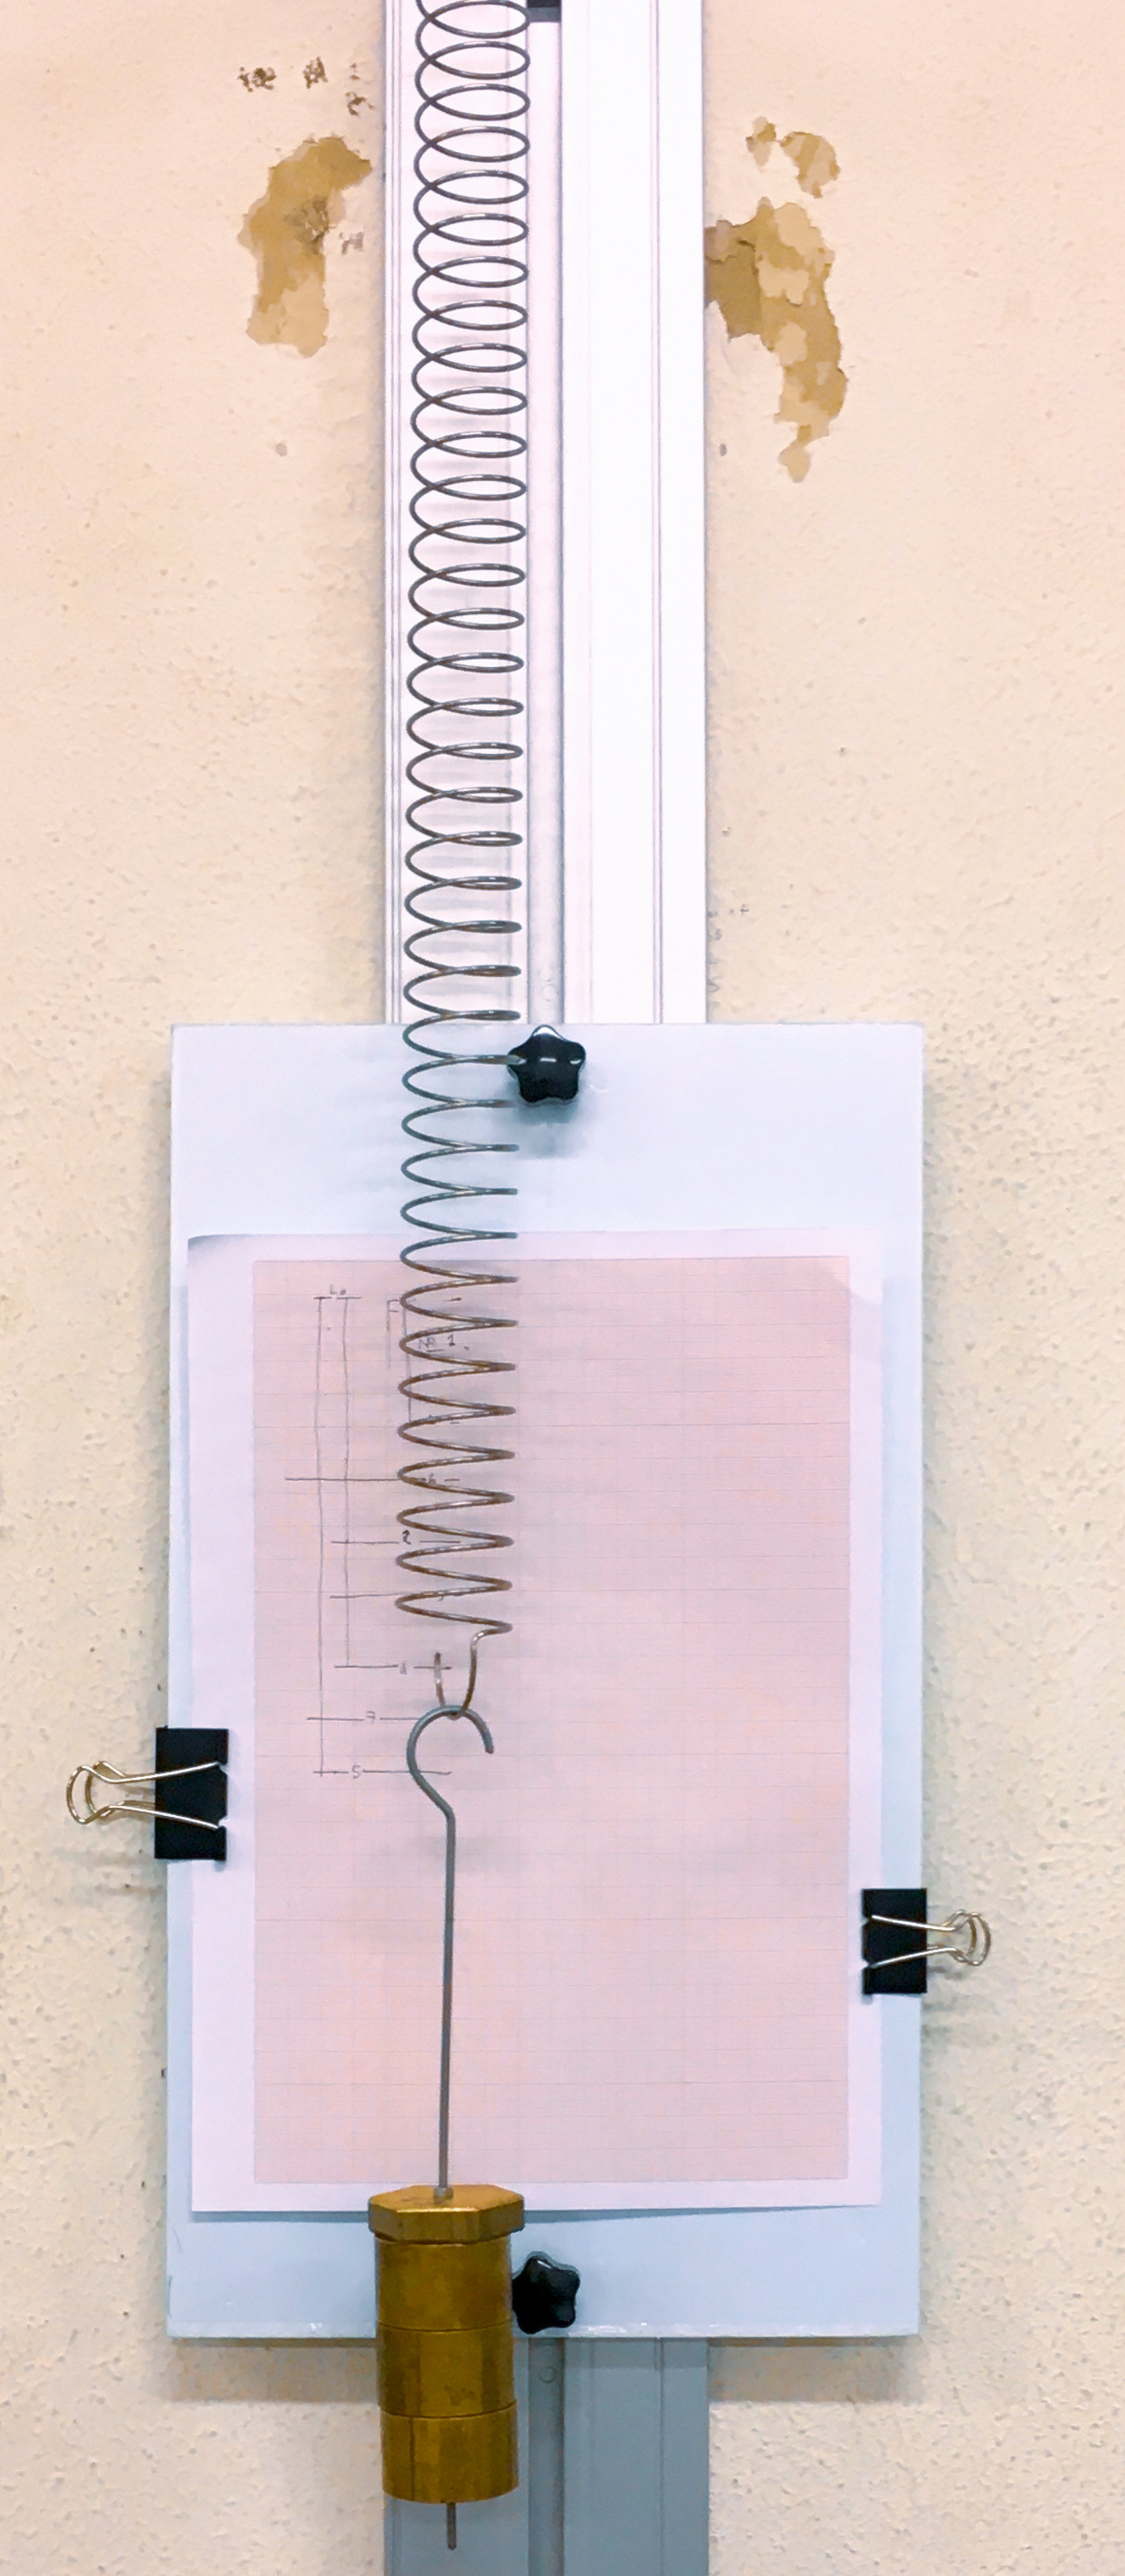
\includegraphics[width=0.72\linewidth]{IMG_0242.JPG}
        \caption{Apparato sperimentale utilizzato nell'esperienza. Sulla guida di alluminio si vede fissato il
        piano di misura con il foglio di carta millimetrata, dove sono riportate le elongazioni dovute alle 
        diverse masse.}
        \label{figure:apparatus}
    \end{figure}

    \begin{figure}[t]
        \centering
        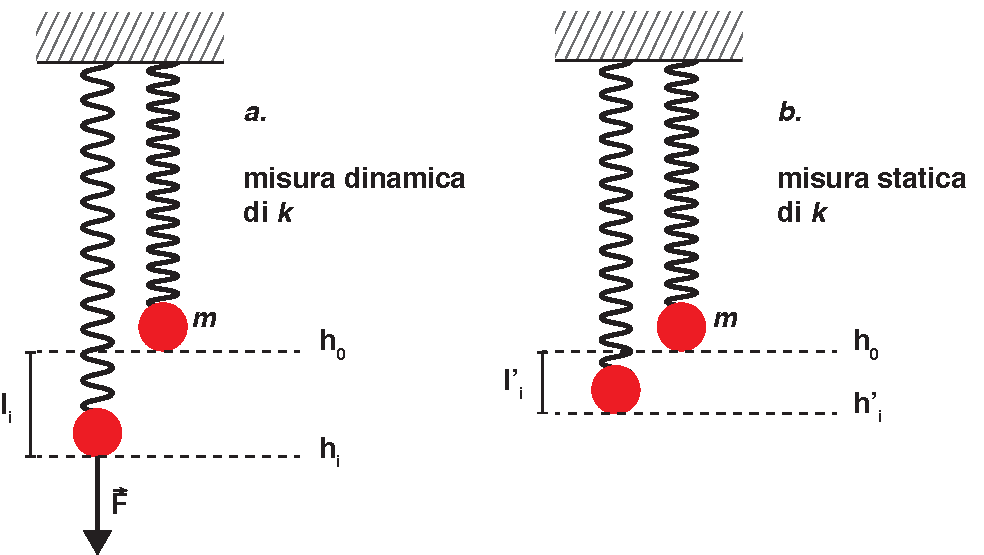
\includegraphics[width=\linewidth]{system_horiz.pdf}
        \label{figure:methods}
        \caption{\textit{a.} Descrizione del metodo di misura dinamico. Al sistema molla + massa \MassI{i} è 
        applicata una forza $\va{F}$, che sposta il sistema dalla sua condizione di equilibrio. Quando viene 
        lasciato andare il sistema si mette in oscillazione attorno alla sua posizione di equilibrio.
        \textit{b.} Descrizione del metodo di misura statico. Alla molla è appesa una massa \MassI{i} che 
        ne causa l'elongazione di una lunghezza \Li{i}$=h_0-h_f$. 
        }
    \end{figure}

    \section{Metodi}
    \label{section:methods}
    Tutte le misure sono riportate nelle unità del Sistema Internazionale (SI). Si assume come nota e costante 
    l'accelerazione di gravità \gLab .

    
    Si fa spesso riferimento anche alla regola del \treSigma, con la quale si vuole intendere la volontà di 
    trasformare un errore di tipo massimo in errore statistico, e quindi considerando il valore vero con una
    probabilità statistica del \treSigma~$\approx99.73\%$ di probabilità del dato vero.\\
    %% MAGARI AGGIUNGERE COMMENTO SU QUANTE CIFRE SI CONSIDERANO E COME APPROSSIMIAMO I VALORI %%
    I valori riportati sono stati approssimati tenendo conto di alcune convenzioni prese. Si approssima 
    l'errore a una cifra significativa se tale cifra è $\geqslant3$, altrimenti se tale cifra è 1 o 2 allora
    si considerano due cifre significative. Considerando quindi le posizioni decimali significative dell'errore
    si approssima per eccesso il valore numerico della grandezza. 

    In entrambi i modelli la molla è sempre utilizzata in un regime elastico, tale per cui la molla è capace
    di ritornare alla condizione iniziale, e quindi in una condizione in cui l'energia totale del sistema si 
    conserva.

    Poiché la portata della bilancia elettronica è di 350~g e le masse da noi utilizzate combinate danno valori
    superiori, procediamo a pesare le masse in combinazioni tali da non superare tale limite della bilancia, 
    ma con lo scopo di non effettuare troppe misure sommate poiché l'errore totale della misura è la somma degli
    errori delle singole pesate. Inoltre per il medesimo motivo il gancio viene pesato in una delle pesate e 
    non singolarmente.

    Per riportare le misure di lunghezza raggiunte dalla molla sul foglio abbiamo utilizzato una squadra per 
    ridurre l'errore dovuto alla parallasse.\\

    Misuriamo la massa della molla utilizzando la squadra come piano d'appoggio per allargare il piatto della 
    bilancia. Tale massa risulta essere $83.894\pm0.004$~g [$= (83.894\pm0.002\text{ stat})$~g].

    Segniamo sul foglio millimetrato la proiezione della lunghezza \Lo raggiunta dalla molla a riposo quando 
    essa è libera senza masse ulteriori appese. 

    \subsection{Metodo Statico}
    \label{subsec:methods_stat}
    Vogliamo ricavare tramite misure di statica un valore \ks (ovvero una misura di $k$).

    Dai pesetti componiamo una massa \MassI{i} tale che la massa rientri nel regime delle elongazioni elastiche 
    per la molla, ovvero che  $0.150 \text{ kg} < m_i < 1.200 \text{ kg}$. 
    Pesata quindi la massa totale (come somma delle diverse pesate) fissiamo sulla vite senza fine tramite i 
    bulloni i pesetti. Agganciamo dunque il sistema composto da masse + gancio alla molla, attendiamo che questa 
    si stabilizzi su una condizione di equilibrio e segniamo sul foglio la lunghezza raggiunta dall'estremo della 
    molla.
    Misuriamo dunque la variazione di elongazione $\delta l_i$, a cui associamo un errore di $\Delta l_i=$1~mm, 
    considerando come incertezza sulla misura il minimo valore misurabile dalla carta millimetrata. Convertiamo 
    poi l'errore assoluto in errore standard $\varepsilon_{l_i} = \Delta l_i /\sqrt{3}$ secondo la regola del 
    \treSigma.
    
    Ripetiamo questo procedimento per sette misure di massa differenti, e trascriviamo i valori in tabella 
    (\reftab{table:raw_data} e \reftab{table:sts_values}).\\ %% <<-------INDICARE TABELLA!!!!!\\

    \begin{figure}
        \centering
        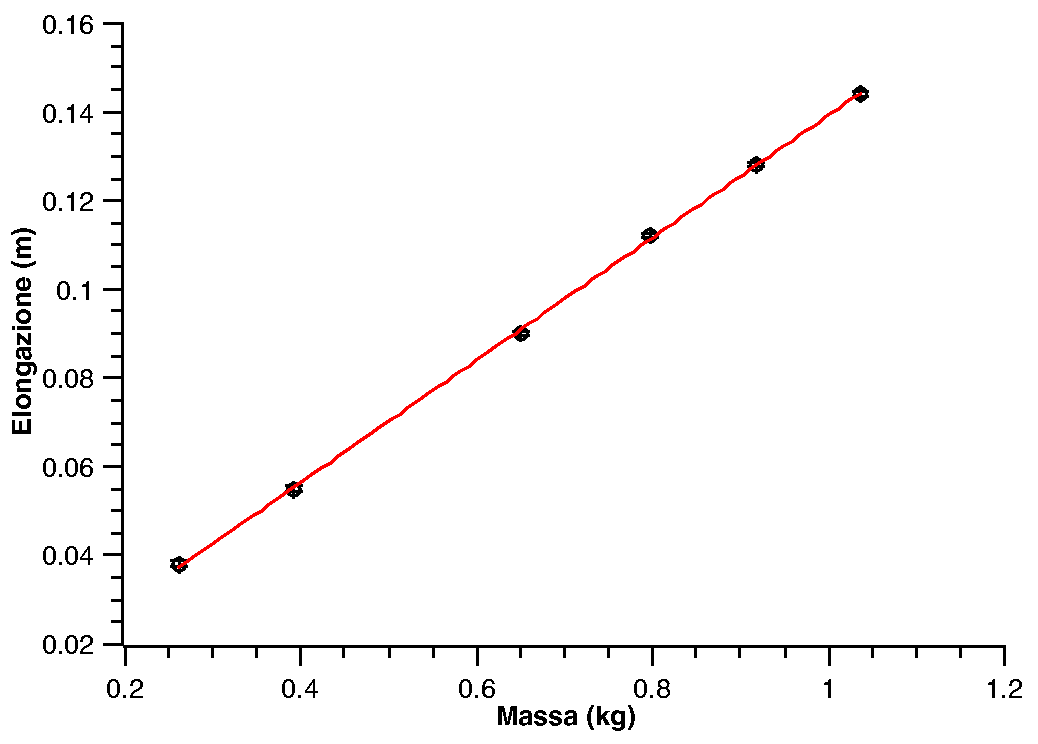
\includegraphics[width=\linewidth]{plot_sts.pdf}
        \caption{Grafico elongazione$\times$massa dove è stato effettuato un fit lineare da cui si è ricavato il 
        valore di \ks. Si potrebbe verificare che la retta individuata passa per l'origine. Possiamo velocemente 
        saggiare la bontà solamente dal rapporto \ChiNdf$=7.328/4\approx1,832$ che è poco più di 1.}
        \label{figure:plot_sts}
    \end{figure}

    Dai valori in \reftab{table:sts_values} possiamo eseguire un grafico lineare elongazione $\times$ massa, come
    in \reffig{figure:plot_sts}. 
    Dal fit eseguito su una funzione del tipo $y=a\cdot x + b$, ricaviamo i valori di $a$ e $b$. Se la relazione 
    che vogliamo dimostrare è della forma \hookeLaw, possiamo concludere che $b\approx0$, e
    $a=\frac{g}{k_{\text{statico}}}$, da cui possiamo ricavare il valore di 
    \misuraIncertezaUM{k_{\text{statico}}}{\varepsilon_k}{}.

    \begin{table}[t]
  \centering
  \footnotesize
  \caption{Valori delle masse e dei relativi allungamenti $\delta l$. L'errore sull'allungamento $\delta l$ è 
  preso considerando la minima variazione misurabile dal foglio di carta millimetrata. Per rendere statistica 
  la misura si è utilizzata la regola del \treSigma e si è così ottenuto il valore di 
  $\varepsilon_{\delta l} = \Delta l / \sqrt{3}$.}
  \label{table:sts_values}
  \begin{tabular}{lcc}
      \hline\hline\\[-1.5ex]
        & Massa                      & Allungamento                            \\[+0.5ex]
        & $m_i\pm\varepsilon_m$ (kg) & $\delta l\pm\varepsilon_{\delta l}$ (m) \\[+0.5ex] \hline \\[-1.5ex]
      1 & $0.261499\pm0.000002$      & $0.0380\pm0.0006$                       \\[+0.5ex]
      2 & $0.650447\pm0.000007$      & $0.0900\pm0.0006$                       \\[+0.5ex]
      3 & $0.796669\pm0.000007$      & $0.1120\pm0.0006$                       \\[+0.5ex]
      4 & $1.035634\pm0.000009$      & $0.1440\pm0.0006$                       \\[+0.5ex]
      5 & $0.393091\pm0.000005$      & $0.0550\pm0.0006$                       \\[+0.5ex]
      6 & $0.916857\pm0.000009$      & $0.1280\pm0.0006$                       \\[+0.5ex]
      \hline \\[-1.5ex]
  \end{tabular}
\end{table}

\begin{table}[t]
    \centering
    \footnotesize
    \caption{Valori delle masse e relativi valori di periodo $\bar{T_i}$. Sono riportati anche i valori di
    $\bar{T_i^2}$. Gli errori relativi ai periodi sono ricavati dal calcolo dell'errore standard ($\varepsilon$). 
    L'errore sulla massa preso dalla linearità dello strumento (0.004 g) è ottenuto dalla somma degli errori dovuti 
    alle diverse pesate. Il valore è poi staticizzato per la regola del \treSigma ($\varepsilon_m = \Delta m/\sqrt{3}$)}
    \label{table:dyn_values}
    \begin{tabular}{lccc}
        \hline\hline\\[-1.5ex]
          & Massa                      & Periodo                         & Periodo al quadrato                       \\[+0.5ex]
          & $m_i\pm\varepsilon_m$ (kg) & $\bar{T_i}\pm\varepsilon_T$ (s) & $\bar{T_i^2}\pm\varepsilon_{T^2}$ (s$^2$) \\[+0.5ex] \hline \\[-1.5ex]
        1 & $0.261499\pm0.000002$      & $0.3761\pm0.0015$               & $0.1415\pm0.0011$                         \\[+0.5ex]
        2 & $0.650447\pm0.000007$      & $0.5646\pm0.0020$               & $0.3188\pm0.0022$                         \\[+0.5ex]
        3 & $0.796669\pm0.000007$      & $0.6217\pm0.0018$               & $0.3865\pm0.0022$                         \\[+0.5ex]
        4 & $1.035634\pm0.000009$      & $0.6962\pm0.0011$               & $0.4847\pm0.0015$                         \\[+0.5ex]
        5 & $0.393091\pm0.000005$      & $0.439 \pm0.003 $               & $0.1925\pm0.0027$                         \\[+0.5ex]
        6 & $0.916857\pm0.000009$      & $0.6574\pm0.0017$               & $0.4322\pm0.0021$                         \\[+0.5ex]
        \hline \\[-1.5ex]
        
    \end{tabular}
\end{table}



    \subsection{Metodo dinamico}
    \label{subsec:methods_dyn}
    Per ogni massa utilizzata nel metodo statico effettuiamo anche una considerazione di tipo dinamico del 
    sistema, per ricavare un valore \kd da confrontare poi con \ks, per verificarne il valore.
    Applichiamo una forza $\va{F}$ al sistema molla + \MassI{i}, spostando la molla dalla sua posizione di 
    equilibrio di un $\delta x$ abbastanza piccolo. Il sistema si metterà dunque in oscillazione. La necessità
    di avere ampiezza piccole può essere spiegata da due fatti: innanzitutto il periodo di oscillazione del 
    sistema non dipende dall'ampiezza dell'oscillazione, e inoltre un ampiezza maggiore porta ad avere una 
    velocità maggiore e quindi, poiché l'attrito viscoso dell'aria è direttamente proporzionale alla velocità 
    $v$ ($\va{f_v}=-\beta \va{v}$) causando quindi uno smorzamento del moto.\\
    Per dimostrare il primo punto, partendo dalle equazioni delle forze in gioco ricaviamo:
    \[
        \va{f_{el}} + \va{P} = M_{\text{tot}}\va{a}
    \]
    da cui 
    \[
        k\cdot x - M\cdot g = - M \cdot \ddot{x}
    \]
    Dividendo per la massa M
    \[
        \frac{k}{M}\cdot x - g = - \ddot{x}
    \]
    Se riscriviamo il termine $\frac{k}{M} \cdot (x - g\cdot\frac{M}{k}) = \xi$, osserviamo che 
    $\ddot{\xi} = \ddot{x}$, quindi possiamo riscrivere come
    \[
        - \frac{k}{M} \cdot \xi = \ddot{\xi}
    \]
    Se consideriamo il fattore $\frac{k}{M}$ questo ha dimensioni {s$^{-1}$\}, quindi possiamo riscrivere
    \[
        - \omega^2_0 \cdot \xi = \ddot{\xi}
    \]
    Che è una equazione differenziale al secondo ordine, che se risolta ci dà proprio l'equazione del moto 
    armonico oscillatorio, dove però il termine $g \cdot \frac{M}{k}$ rappresenta la posizione $x_{\text{eq}}$
    di equilibrio. Da $\omega_0 = \sqrt{k/M}$ possiamo ricavare il periodo di oscillazione del sistema.\\
    Se infatti il periodo è $T = \frac{2 \pi}{\omega_0}$, allora otteniamo
    \[
        T = 2 \pi \sqrt{\frac{M}{k}}
    \]
    che denota la non dipendenza del periodo dall'ampiezza di oscillazione. 

    Con il cronometro misuriamo il periodo di 10 oscillazioni (\Ti{10\times1\times i}). Ripetiamo la misurazione
    per 10 volte, ottenendo quindi \Ti{10\times1\times i}, \Ti{10\times2\times i}, \ldots , 
    \Ti{10\times10\times i}.\\
    Cambiamo la massa e ripetiamo le stesse misure, ottenendo i valori riportati in tabella in fondo al 
    documento (\reftab{table:raw_data}). In \reftab{table:dyn_values} non sono riportati i valori del punto 2, e 
    quindi gli altri valori sono fatti scalare, poiché come si illustra dopo, tale punto è ritenuto essere erroneo
    e quindi eliminato per considerazioni successive.%% <<--- 

    Cronometriamo 10 oscillazioni per ridurre l'errore di reazione dividendolo su più oscillazioni, dalle 
    quali ricaviamo poi il periodo di una singola oscillazione $T_{1\times i} = T_{10\times1\times i}/10$, \ldots ,
    $T_{10\times i} = T_{10\times10\times i}/10$.
    Dai valori $T_{1\times i}$, \ldots, $T_{10\times i}$ possiamo inoltre eseguire una analisi statistica e 
    ricavare un valore medio $\bar{T}_i$ e l'errore standard associato ricavato come 
    $\varepsilon_T = \frac{S_{10}}{\sqrt{10}}$. 
    
    Trascriviamo i valori così ricavati in \reftab{table:dyn_values}.

    \begin{figure}
        \centering
        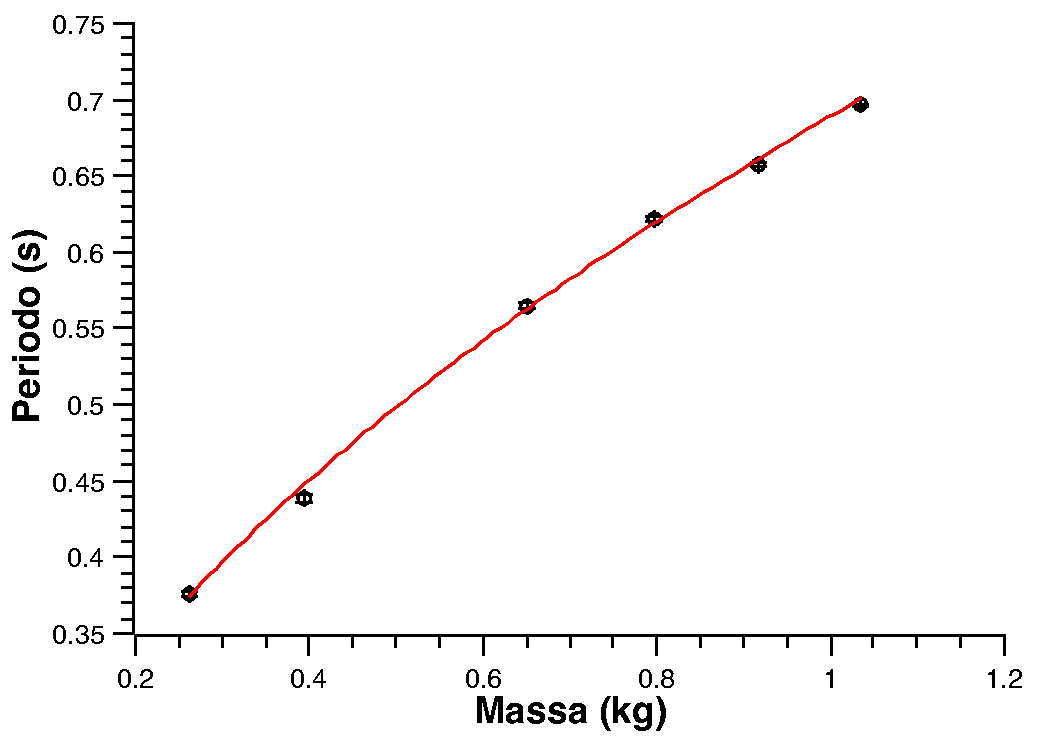
\includegraphics[width=\linewidth]{plot_dyn.pdf}
        \caption{Grafico periodo$\times$massa. Il fit è stato ottenuto a partire da una funzione uguale a quella
        del periodo $T = 2 \pi \sqrt{\left(M+(m_{\text{molla}})/(3)\right)/\left(k\right)}$. Si può osservare un 
        andamento parabolico della curva, in accordo con la teoria.}
        \label{figure:plot_dyn}
    \end{figure}

    \begin{figure}
        \centering
        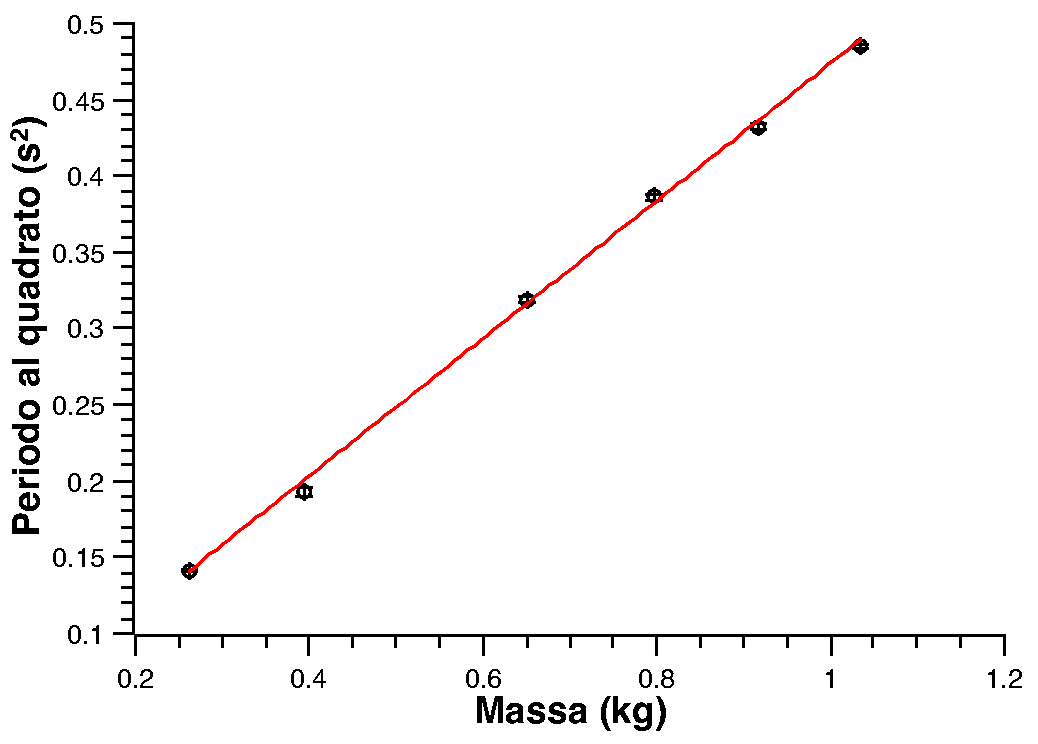
\includegraphics[width=\linewidth]{plot_dyn_lin.pdf}
        \caption{Grafico periodo$^2\times$massa. Il fit è stato eseguito a partire da una relazione lineare come 
        descritto nel paragrafo dei metodi \ref{subsec:methods_dyn}.}
        \label{figure:plot_dyn_lin}
    \end{figure}

    La relazione che lega il periodo $T$ alla massa, come ricavato in precedenza è
    \[
        T = 2 \pi \sqrt{\frac{M}{k}}
    \]
    la formula presentata è valida però solo per un sistema composto da una molla ideale di massa trascurabile, 
    ma nel nostro caso il valore della massa della molla è di $0.083894\pm0.000004$~kg, quindi non trascurabile 
    rispetto alle masse considerate.
    Si trova necessario introdurre quindi un termine correttivo che tenga conto dell'influenza della massa della
    molla:
    \[
        T = 2 \pi \sqrt{\frac{M+\frac{m_{\text{molla}}}{3}}{k}}
    \]
    
    Se eseguiamo il grafico periodo$\times$massa dovremmo individuare un andamento parabolico con l'asse sull'asse 
    delle masse. Osservando infatti la \reffig{figure:plot_dyn} si può vedere chiaramente un andamento che rispetta
    la legge sopra descritta.

    Procediamo ora con la linearizzazione della relazione del periodo. Partendo dalla formula
    \[
        T = 2 \pi \sqrt{\frac{M+\frac{m_{\text{molla}}}{3}}{k}}
    \]
    otteniamo elevando al quadrato ambo i membri
    \[
        T^2 = \frac{4 \pi^2}{k_{\text{dinamico}}} \cdot M + \frac{4 \pi^2 \cdot 
        \frac{m_{\text{molla}}}{3}}{k_{\text{dinamico}}}
    \]
    ovvero ponendo $a'=\frac{4 \pi^2}{k_{\text{dinamico}}}$ e 
    $b'=\frac{4 \pi^2 \cdot \frac{m_{\text{molla}}}{3}}{k_{\text{dinamico}}}$ possiamo riscriverla come 
    $T^2 = a'\cdot M + b'$, 
    dove $M=m_i$ è la massa che agganciamo alla molla.

    Ricaviamo $\bar{T_i^2}$ da $\bar{T_i}$ eseguendo un semplice elevamento a potenza ($\bar{T_i^2}=
    (\bar{T_i})^2$).
    Ricaviamo l'errore standard sul periodo al quadrato $\varepsilon_{T^2} = 2~\cdot~\bar{T_i}~\cdot~
    \varepsilon_{T}$.

    Partendo dai dati presenti in \reftab{table:dyn_values} dei valori di $m_i\pm\varepsilon_m$ e 
    $\bar{T_i^2}\pm\varepsilon_{T^2}$ possiamo rappresentarli nel grafico in \reffig{figure:plot_dyn_lin}.
    Su questi punti possiamo eseguire un fit lineare con una funzione $y = a'\cdot x + b'$, da cui ricaviamo i 
    valori dei parametri $a'$ e $b'$.

    \section{Risultati}
    \label{section:results}

    \subsection{Risultati metodo statico}
    \label{subsec:results_sts}
    Dal fit lineare della funzione $y=ax+b$ otteniamo i valori dei parametri $a$ e $b$ con i rispettivi errori 
    standard $\varepsilon_a$ e $\varepsilon_b$ ($a = 0.1380\pm0.0009$ m/kg, $b = 0.0013\pm0.0006$ m).\\
    Nel paragrafo \ref{subsec:methods_stat} abbiamo ottenuto che $a=\frac{g}{k_{\text{statico}}}$ e $b\approx0$.
    Verifichiamo innanzitutto che $b$ sia compatibile con zero attraverso la relazione
    \[
        \left|b-0\right|<3\sqrt{\varepsilon_b^{2}+\varepsilon_0^{2}}
    \]
    ma, poiché stiamo cercando la compatibilità con lo zero abbiamo che 
    \[
        \left|b\right|<3\sqrt{\varepsilon_b^{2}}
    \]
    ovvero, per $b=0.0013\pm0.0006$ m abbiamo che la relazione $0.0013~<~3~\cdot~0.0006$ è verificata
    ($0.00128<0.00186$).\\
    Da $a$ invece possiamo ricavare il valore di \ks: infatti se $a=\frac{g}{k_{\text{statico}}}$, allora 
    \[
        k_{\text{statico}} = \frac{g}{a} = 71.1 \text{ N/m}
    \]
    dove $g=$\gLab noto con errore statistico. Ricaviamo quindi \ks=$71.1$ N/m, e possiamo ricavare l'errore 
    \[
        \varepsilon_k = \sqrt{\left(\frac{\varepsilon_g}{a}\right)^2+\left(-\frac{g\cdot\varepsilon_a}
        {a^2}\right)^2} = 0.4 \text{ N/m} 
    \]
    Quindi il valore di \ks$=71.1\pm0.4$ N/m, che riportiamo anche in \reftab{table:results}.

    \subsection{Risultati metodo dinamico}
    \label{subsec:results_dyn}

    Dal fit lineare della funzione $y=a'x+b'$ otteniamo i valori di $a'\pm\varepsilon_{a'} = 0.4506\pm0.0016$ m/N
    e $b'\pm\varepsilon_{b'} = 0.0230\pm0.0024$ s$^2$.
    Poiché $T^2 = y$ e $m_i = x$, allora possiamo riscrivere $T^2~=~a'm_i~+~b'$, ovvero 
    $a' = \frac{4\pi^2}{k_{\text{dinamico}}}$ e $b' = \frac{4\pi^2m_{\text{molla}}}{3k_{\text{dinamico}}}$.

    Possiamo dunque ricavarci \kd$\pm\varepsilon_k$
    \[
        k_{\text{dinamico}} = \frac{4\pi^2}{a'} = 87.6 \text{ N/m}
    \] 
    con il relativo errore standard 
    \[
        \varepsilon_k = \sqrt{\left(-\frac{4\pi^2}{a^2}\right)^2\cdot\varepsilon_{a'}^2} = 0.3\text{ N/m}  
    \]
    e possiamo anche ricavarci il valore della massa $m_{\text{molla}}\pm\varepsilon_m$
    \[
        m_{\text{molla}} = \frac{3\cdot b'\cdot k_{\text{dinamico}}}{4\pi^2} = \frac{3\cdot b'}{a'} = 0.153 
        \text{ kg}
    \]
    e il relativo errore standard
    \[
        \varepsilon_m = \sqrt{\left(\frac{3}{a'}\right)^2\cdot\varepsilon_{b'}^2 + \left(\frac{3\cdot b'}
        {{a'}^2}\right)^2\cdot\varepsilon_{a'}^2} = 0.016 \text{ kg}
    \]
    Trascriviamo quindi i valori di \kd$ = 87.6\pm0.3$ N/m e $m_{\text{molla}} = 0.153\pm0.016$ kg in 
    \reftab{table:results}.

    \begin{table}[h!]
    \centering
    \footnotesize
    \caption{Risultati ottenuti dall'analisi effettuata nel paragrafo \ref{section:results}. I valori sono 
    riportati con il loro errore statistico ricavato tramite propagazione degli errori. Dai due diversi metodi sono
    anche calcolati due grandezze differenti: l'offset, ovvero la distanza della funzione di fit dall'origine (per il metodo 
    statico), e il valore della massa della molla, per il metodo dinamico.}
    \label{table:results}
    \begin{tabular}{lccc}
        \hline\hline\\[-1.5ex]
        Metodo   & $k\pm\varepsilon_k$ (N/m) & err. rel. &                                                            \\[+0.5ex] \hline \\[-1.5ex]
        Statico  & $71.1\pm0.4$              & 0.6 \%    & offset $\delta\pm\varepsilon_{\delta} = 0.0013\pm0.0006$ m \\[+0.5ex]
        Dinamico & $87.6\pm0.3$              & 0.3 \%    & $m_{\text{molla}}\pm\varepsilon_m = 0.153\pm.016$ kg       \\[+0.5ex]
        \hline \\[-1.5ex]

    \end{tabular}
\end{table}

    \section{Conclusione}
    \label{section:conclusion}

    Abbiamo verificato che l'andamento sperimentale del rapporto dell'elongazione sulla massa applicata alla molla 
    è costante, come affermato dalla relazione \hookeLaw.
    Allo stesso modo abbiamo osservato un comportamento della relazione tra periodo e massa appesa al sistema che 
    bene può essere descritto dalla relazione
    \[
        T = 2\pi \sqrt{\frac{M}{k}}  
    \]
    Possiamo perciò procedere a studiare quantitativamente i valori ottenuti, e confrontare tra loro i risultati 
    dei due modelli presi in analisi.

    

    \begin{figure*}
        \centering
        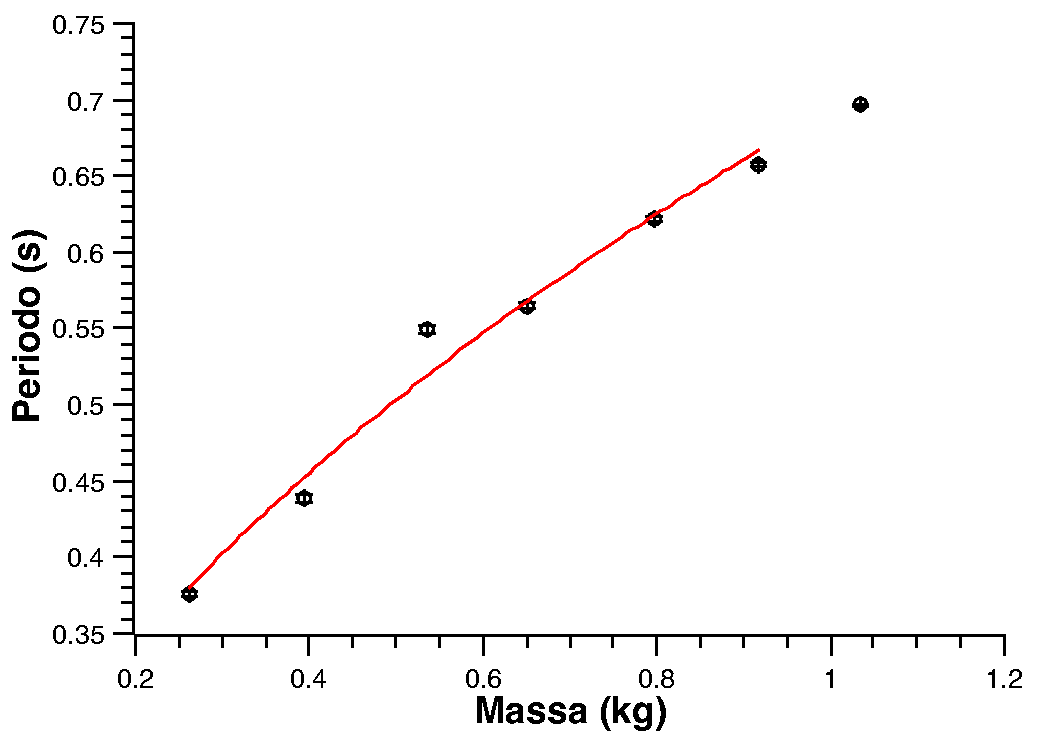
\includegraphics[width=0.45\linewidth]{plot_dyn_2.pdf}
        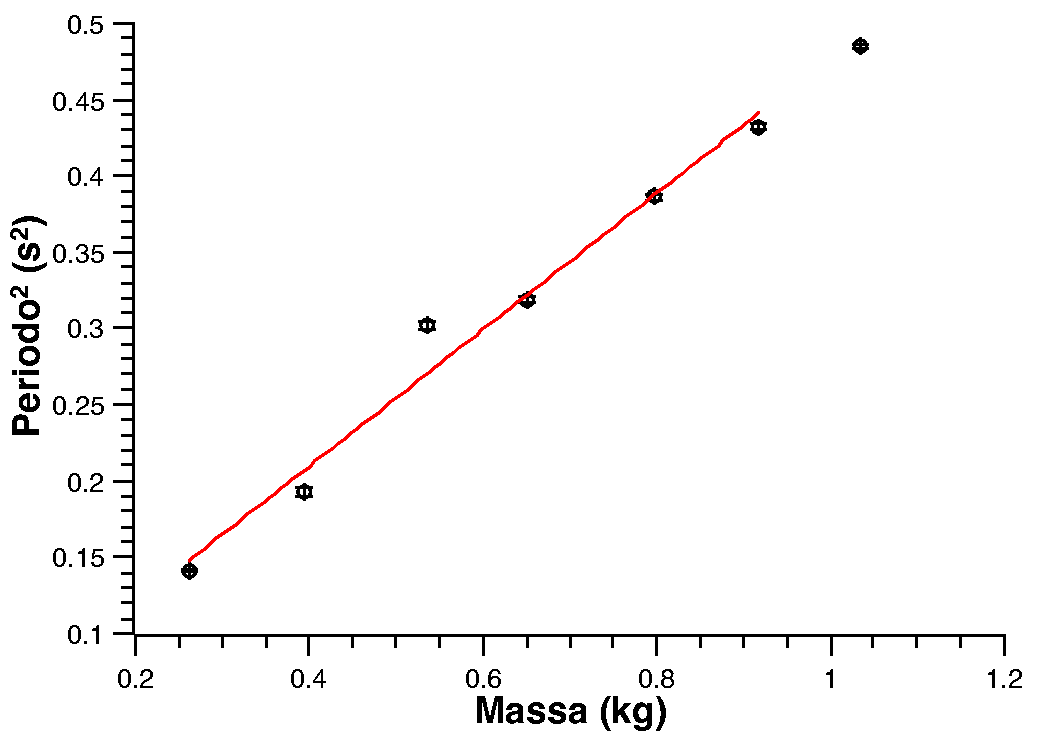
\includegraphics[width=0.45\linewidth]{plot_dyn_lin_2.pdf}
        \caption{Grafici periodo$\times$massa e periodo$^2\times$massa dove sono stati presi in considerazione 
        tutti e sette i punti, denotando quindi lo scostamento~>~\treSigma del valore del terzo punto da un teorico 
        fit, in rosso.}
        \label{figure:plot_2}
    \end{figure*}

    \setcounter{table}{0}
    \renewcommand{\thetable}{A\arabic{table}}
    %% this file is for all the tables that go in the appendix as additional data
\begin{table*}[t!]
    \centering
    \caption{Dati grezzi relativi alle misure di massa per ogni $i$-esima masse e le misure del periodo di 
    oscillazione e della elongazione associate alla $i$-esima massa.}
    \footnotesize
    \label{table:raw_data}
    \begin{tabular}{l*{7}{c}}
        \hline\hline\\[-1.5ex]
                                 & \multicolumn{7}{c}{Misure di massa (kg) (errore assoluto $\pm4\times10^{-6}$ kg per ogni pesata)}            \\[+0.5ex] \hline \\[-1.5ex]
        $m_i$                    & 0.261499 & 0.535073 & 0.650447 & 0.796669 & 1.035634 & 0.393091 & 0.916857                                   \\[+0.5ex]
        $\delta m$               & 0.000004 & 0.000008 & 0.000012 & 0.000012 & 0.000016 & 0.000008 & 0.000016                                   \\[+0.5ex] \hline \\[-1.5ex]
                                 & \multicolumn{7}{c}{Periodi di 10 oscillazioni presi 10 volte per ogni massa (metodo dinamico) (s)}           \\[+0.5ex]
                                 & \multicolumn{7}{c}{\Ti{10\times n\times 1}, \ldots , \Ti{10\times n\times 7} (errore assoluto $\pm 0.01$ s)} \\[+0.5ex] \hline \\[-1.5ex]
        $T_{10\times1 \times i}$ & 3.75     & 5.52     & 5.58     & 6.25     & 7.01     & 4.50     & 6.65                                       \\[+0.5ex]
        $T_{10\times2 \times i}$ & 3.83     & 5.52     & 5.70     & 6.27     & 6.94     & 4.25     & 6.58                                       \\[+0.5ex]
        $T_{10\times3 \times i}$ & 3.71     & 5.58     & 5.59     & 6.16     & 6.93     & 4.34     & 6.63                                       \\[+0.5ex]
        $T_{10\times4 \times i}$ & 3.83     & 5.37     & 5.77     & 6.22     & 6.94     & 4.51     & 6.57                                       \\[+0.5ex]
        $T_{10\times5 \times i}$ & 3.78     & 5.38     & 5.62     & 6.12     & 6.91     & 4.26     & 6.57                                       \\[+0.5ex]
        $T_{10\times6 \times i}$ & 3.70     & 5.53     & 5.66     & 6.31     & 7.00     & 4.33     & 6.51                                       \\[+0.5ex]
        $T_{10\times7 \times i}$ & 3.76     & 5.60     & 5.70     & 6.19     & 7.00     & 4.37     & 6.46                                       \\[+0.5ex]
        $T_{10\times8 \times i}$ & 3.78     & 5.53     & 5.63     & 6.19     & 6.96     & 4.44     & 6.59                                       \\[+0.5ex]
        $T_{10\times9 \times i}$ & 3.71     & 5.50     & 5.58     & 6.26     & 6.95     & 4.37     & 6.59                                       \\[+0.5ex]
        $T_{10\times10\times i}$ & 3.76     & 5.44     & 5.63     & 6.20     & 6.98     & 4.50     & 6.59                                       \\[+0.5ex] \hline \\[-1.5ex]
                                 & \multicolumn{7}{c}{Elongazioni (metodo statico) (m) (errore assoluto $\pm1\times10^{-3}$ m)}                 \\[+0.5ex] \hline \\[-1.5ex]
        $l_i$                    & 0.038    & 0.074    & 0.090    & 0.112    & 0.144    & 0.055    & 0.128                                      \\[+0.5ex]
        \hline \\[-1.5ex]
    \end{tabular}
\end{table*}


    \subsection{Controlli}

    Abbiamo già verificato la compatibilità di zero del valore di offset $b\pm\varepsilon_b =
    \delta\pm\varepsilon_{\delta}$
    nel paragrafo \ref{subsec:results_sts}.\\
    Procediamo a verificare la compatibilità del valore misurato della massa della molla 
    $m_{\text{molla}}^t\pm\varepsilon_m^t = (0.083893\pm0.000002\text{ stat})$ kg con il valore trovato 
    sperimentalmente $m_{\text{molla}}^s\pm\varepsilon_m^s = (0.153\pm0.016\text{ stat})$:
    \[
        \left|m_{\text{molla}}^t-m_{\text{molla}}^s\right|<3\cdot\sqrt{\left(\varepsilon_m^t\right)^2 + 
        \left(\varepsilon_m^s\right)^2}
    \]
    \[
        \left|0.083893-0.153\right|<3\cdot\sqrt{\left(0.000002\right)^2 + \left(0.016\right)^2} 
        \to 0.07<0.05\text{ kg}
    \]
    che è una relazione falsa, quindi le masse non sono compatibili.

    Procediamo infine a verificare la compatibilità dei valori di \kd e \ks:
    \[
        \left|k_{\text{dinamico}}-k_{\text{statico}}\right|<3\cdot\sqrt{\left(\varepsilon_k^d\right)^2 + 
        \left(\varepsilon_k^s\right)^2} \to
    \]
    \[
        \to 16.5<1.5 \text{ N/m}
    \]
    che mostra la non compatibilità dei risultati.

    \subsection{Possibili errori sistematici, considerazioni finali}
    La seconda colonna di valori della \reftab{table:results} è stata eliminata per la trattazione dettagliata 
    e l'analisi dei dati poiché, come si osserva in \reffig{figure:plot_2} il terzo punto, che è rappresentato dai 
    valori della seconda colonna, risulta essere più di \treSigma distante dal valore del fit.\\
    Abbiamo perciò deciso di non considerarlo nell'analisi dettagliata, e infatti non è stato riportato in 
    \reftab{table:sts_values} e \reftab{table:dyn_values}.\\

    Pur ricontrollando i calcoli eseguiti e le analisi effettuate, il valore di \kd e quello di \ks non risultano 
    essere compatibili. Non possiamo però discriminare quale dei due valori sia più attendibile e quale porti 
    invece un errore.\\
    Le misure statiche possono essere ricontrollate dal foglio di carta millimetrata, quindi, a meno di un errore 
    sistematico nel segnare il punto sul foglio, possiamo però ritenere meno probabili errori legati alla misura
    statica. 
    L'errore potrebbe essere perciò legato alla strumentazione, anche se riteniamo che non possa essere causato
    dalla bilancia, in quanto è stata utilizzata per entrambi i metodi.\\
    Potrebbe esserci stato anche un errore sistematico dovuto allo strumento di misura del tempo, il cronometro 
    elettronico, ma non possiamo però verificare effettivamente quale sia la causa di questa discrepanza.\\
    Possiamo pensare che l'errore sia legato più probabilmente alla misura dinamica anche da un veloce confronto 
    dei valori dei rapporti \ChiNdf dei due fit per i due modelli: per il modello statico infatti \ChiNdf
    $= 7.328/4\approx1.8$, che rappresenta una buona stima del fit, essendo molto vicino a 1,
    mentre per il modello dinamico \ChiNdf$= 37.235/4\approx9.3$, che rappresenta un fit che seppur probabile,
    è più incerto del fit eseguito sul modello statico.


    \appendix
    
    \section{Dati completi}
    %%includere tabelle dati completi periodi e calcolo periodi.
    Riportiamo in forma tabulare in \reftab{table:raw_data} i dati raccolti relativi alle masse, ai periodi e alle 
    elongazioni per tutte le misure effettuate.



\end{document}
    
